\documentclass[11pt,letterpaper]{report}

% ============================================================================
% PACKAGES
% ============================================================================
\usepackage[utf8]{inputenc}
\usepackage[T1]{fontenc}
\usepackage[margin=1in,headheight=14pt]{geometry}
\usepackage{graphicx}
\usepackage{xcolor}
\usepackage{tikz}
\usetikzlibrary{shapes,arrows,positioning,calc,shadows,decorations.pathmorphing,mindmap,trees}
\usepackage{booktabs}
\usepackage{longtable}
\usepackage{array}
\usepackage{tabularx}
\usepackage{multirow}
\usepackage{enumitem}
\usepackage{fancyhdr}
\usepackage{titlesec}
\usepackage{tcolorbox}
\tcbuselibrary{skins,breakable}
\usepackage{amsmath}
\usepackage{amssymb}
\usepackage{hyperref}
\usepackage{cleveref}
\usepackage{siunitx}
\usepackage{float}
\usepackage{parskip}
\usepackage{pifont}

% Define simple icon replacements
\newcommand{\faRocket}{$\blacktriangleright$}
\newcommand{\faCogs}{$\diamond$}
\newcommand{\faFlag}{$\star$}
\newcommand{\faMicrochip}{$\circ$}
\newcommand{\faExclamationTriangle}{$\triangle$}
\newcommand{\faStar}{$\star$}
\newcommand{\faLayerGroup}{$\square$}

% ============================================================================
% COLOR DEFINITIONS
% ============================================================================
\definecolor{primaryblue}{RGB}{0,74,127}
\definecolor{secondaryblue}{RGB}{70,130,180}
\definecolor{accentgold}{RGB}{196,154,0}
\definecolor{successgreen}{RGB}{46,139,87}
\definecolor{warningorange}{RGB}{230,126,34}
\definecolor{dangered}{RGB}{192,57,43}
\definecolor{lightblue}{RGB}{230,240,250}
\definecolor{lightgreen}{RGB}{230,250,230}
\definecolor{lightyellow}{RGB}{255,250,230}
\definecolor{lightpurple}{RGB}{240,230,250}
\definecolor{lightgray}{RGB}{248,248,248}
\definecolor{phase1color}{RGB}{52,152,219}
\definecolor{phase2color}{RGB}{155,89,182}
\definecolor{phase3color}{RGB}{46,204,113}
\definecolor{phase4color}{RGB}{230,126,34}
\definecolor{phase5color}{RGB}{231,76,60}

% ============================================================================
% TCOLORBOX CONFIGURATIONS
% ============================================================================

\newtcolorbox{visionbox}{
    colback=lightblue,
    colframe=primaryblue,
    title={\faRocket\ Vision Statement},
    fonttitle=\bfseries\large,
    breakable,
    enhanced,
    left=8pt,
    right=8pt,
    top=6pt,
    bottom=6pt
}

\newtcolorbox{techbox}{
    colback=lightgray,
    colframe=secondaryblue,
    title={\faCogs\ Technical Requirements},
    fonttitle=\bfseries,
    breakable,
    enhanced,
    left=8pt,
    right=8pt
}

\newtcolorbox{milestonebox}[1][]{
    colback=lightyellow,
    colframe=accentgold,
    title={\faFlag\ #1},
    fonttitle=\bfseries,
    breakable,
    enhanced,
    left=8pt,
    right=8pt
}

\newtcolorbox{circuitbox}[1][]{
    colback=lightgreen,
    colframe=successgreen,
    title={\faMicrochip\ #1},
    fonttitle=\bfseries,
    breakable,
    enhanced,
    left=8pt,
    right=8pt
}

\newtcolorbox{warningbox}{
    colback=lightyellow,
    colframe=warningorange,
    title={\faExclamationTriangle\ Critical Consideration},
    fonttitle=\bfseries,
    breakable,
    enhanced,
    left=8pt,
    right=8pt
}

\newtcolorbox{phasebox}[2][primaryblue]{
    colback=white,
    colframe=#1,
    title={#2},
    fonttitle=\bfseries\Large,
    boxrule=2pt,
    arc=4pt,
    left=10pt,
    right=10pt,
    top=10pt,
    bottom=10pt,
    before skip=15pt,
    after skip=15pt,
    shadow={2pt}{-2pt}{0pt}{black!20}
}

% ============================================================================
% HEADER/FOOTER CONFIGURATION
% ============================================================================
\pagestyle{fancy}
\fancyhf{}
\fancyhead[L]{\textsl{\leftmark}}
\fancyhead[R]{\textsl{AoE Circuit Simulator Roadmap}}
\fancyfoot[C]{\thepage}
\renewcommand{\headrulewidth}{0.4pt}
\renewcommand{\footrulewidth}{0.4pt}

% ============================================================================
% TITLE FORMATTING
% ============================================================================
\titleformat{\chapter}[display]
    {\normalfont\huge\bfseries\color{primaryblue}}
    {\chaptertitlename\ \thechapter}{20pt}{\Huge}
\titleformat{\section}
    {\normalfont\Large\bfseries\color{primaryblue}}
    {\thesection}{1em}{}
\titleformat{\subsection}
    {\normalfont\large\bfseries\color{primaryblue!80!black}}
    {\thesubsection}{1em}{}
\titleformat{\subsubsection}
    {\normalfont\normalsize\bfseries\color{primaryblue!60!black}}
    {\thesubsubsection}{1em}{}

% ============================================================================
% HYPERREF CONFIGURATION
% ============================================================================
\hypersetup{
    colorlinks=true,
    linkcolor=primaryblue,
    citecolor=successgreen,
    urlcolor=secondaryblue,
    hypertexnames=false,
    pdftitle={The Art of Electronics Circuit Simulator - Development Roadmap},
    pdfauthor={Circuit Simulation Project},
    pdfsubject={Web-Based Electronics Education Platform},
    pdfkeywords={electronics, simulation, SPICE, web application, education}
}

% ============================================================================
% CUSTOM COMMANDS
% ============================================================================
\newcommand{\aoe}{\textit{The Art of Electronics}}
\newcommand{\xchapters}{\textit{The X Chapters}}
\newcommand{\milestone}[1]{\textcolor{accentgold}{\faFlag\ \textbf{#1}}}
\newcommand{\priority}[1]{\textcolor{dangered}{\faStar\ Priority: #1}}
\newcommand{\complexity}[1]{\textcolor{secondaryblue}{\faLayerGroup\ Complexity: #1}}
\newcommand{\mycheck}{\textcolor{successgreen}{\ding{51}}}
\newcommand{\mycross}{\textcolor{dangered}{\ding{55}}}

% ============================================================================
% DOCUMENT BEGIN
% ============================================================================
\begin{document}

% ============================================================================
% TITLE PAGE
% ============================================================================
\begin{titlepage}
    \centering
    \vspace*{0.5cm}
    
    \begin{tikzpicture}[remember picture, overlay]
        \fill[primaryblue] (current page.north west) rectangle ([yshift=-5cm]current page.north east);
        \fill[accentgold] ([yshift=-5cm]current page.north west) rectangle ([yshift=-5.4cm]current page.north east);
    \end{tikzpicture}
    
    \vspace{3cm}
    
    {\Huge\bfseries\color{primaryblue} The Art of Electronics\\[0.3cm]}
    {\LARGE\bfseries\color{primaryblue!80!black} Interactive Circuit Simulator\\[0.5cm]}
    
    \vspace{0.5cm}
    
    {\Large\color{secondaryblue} Comprehensive Development Roadmap\\[0.2cm]}
    {\large Web Application for Circuit Simulation \& Education}
    
    \vspace{1.5cm}
    
    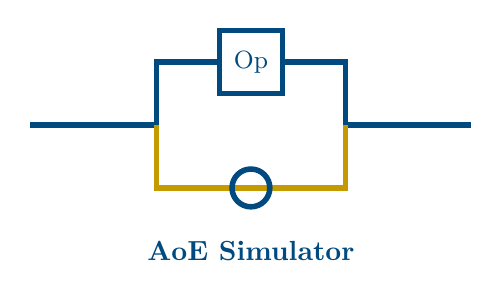
\begin{tikzpicture}[scale=0.8]
        % Simplified circuit schematic icon
        \draw[primaryblue, line width=2pt] (0,0) -- (2,0);
        \draw[primaryblue, line width=2pt] (2,0) -- (2,1) -- (3,1);
        \draw[primaryblue, line width=2pt, fill=white] (3,0.5) rectangle (4,1.5);
        \node[primaryblue] at (3.5,1) {\small Op};
        \draw[primaryblue, line width=2pt] (4,1) -- (5,1) -- (5,0) -- (7,0);
        \draw[accentgold, line width=2pt] (2,0) -- (2,-1) -- (5,-1) -- (5,0);
        \draw[primaryblue, line width=2pt] (3.5,-1) circle (0.3);
        \node at (3.5,-2) {\color{primaryblue}\textbf{AoE Simulator}};
    \end{tikzpicture}
    
    \vspace{1.5cm}
    
    \begin{tcolorbox}[
        colback=lightblue,
        colframe=primaryblue,
        width=0.85\textwidth,
        arc=3mm,
        boxrule=1pt
    ]
    \centering
    \textbf{Project Scope:}\\[0.2cm]
    A comprehensive web-based circuit simulation platform covering all circuits\\
    from \aoe{} (3rd Edition) and \xchapters{}\\[0.2cm]
    \textbf{Total Circuits:} 150+ unique simulation modules\\
    \textbf{Estimated Timeline:} 18--24 months full development
    \end{tcolorbox}
    
    \vfill
    
    {\large\textbf{Version:} 1.0}\\[0.3cm]
    {\large\textbf{Date:} \today}
    
    \vspace{0.5cm}
    
    \begin{tikzpicture}[remember picture, overlay]
        \fill[accentgold] (current page.south west) rectangle ([yshift=0.4cm]current page.south east);
        \fill[primaryblue] ([yshift=0.4cm]current page.south west) rectangle ([yshift=1.2cm]current page.south east);
    \end{tikzpicture}
    
\end{titlepage}

% ============================================================================
% TABLE OF CONTENTS
% ============================================================================
\tableofcontents
\clearpage

% ============================================================================
% EXECUTIVE SUMMARY
% ============================================================================
\chapter{Executive Summary}
\label{ch:executive_summary}

\begin{visionbox}
This roadmap outlines the development of a comprehensive web-based circuit simulation platform designed to accompany \aoe{} by Paul Horowitz and Winfield Hill, including both the main text (3rd Edition) and \xchapters{}. The platform will provide interactive, browser-based simulations of every circuit covered in the companion laboratory curricula, enabling learners to explore electronics concepts through hands-on virtual experimentation.
\end{visionbox}

\section{Project Objectives}

The AoE Circuit Simulator aims to achieve the following primary objectives:

\begin{enumerate}[leftmargin=*, itemsep=6pt]
    \item \textbf{Comprehensive Coverage:} Simulate all circuits from both the main AoE curriculum (Phases 0--6) and the X Chapters advanced curriculum (Projects A1--A5, D1--D2, E1--E2), totaling over 150 distinct circuit configurations.
    
    \item \textbf{Educational Integration:} Align simulations directly with the laboratory curriculum structure, providing guided exercises, measurement challenges, and theoretical verification opportunities.
    
    \item \textbf{Accurate Simulation:} Implement SPICE-accurate simulation engines for analog circuits, logic simulation for digital circuits, and hybrid simulation for mixed-signal systems.
    
    \item \textbf{Accessible Platform:} Deliver simulations via modern web browsers without requiring software installation, plugin downloads, or high-performance hardware.
    
    \item \textbf{Interactive Learning:} Provide virtual oscilloscopes, multimeters, spectrum analyzers, and other measurement tools that mirror real laboratory equipment.
\end{enumerate}

\section{Source Material Summary}

The development roadmap draws from two comprehensive laboratory curricula:

\begin{table}[H]
\centering
\caption{Source Curriculum Overview}
\label{tab:source_overview}
\begin{tabularx}{\textwidth}{@{}lXl@{}}
\toprule
\textbf{Curriculum} & \textbf{Focus Areas} & \textbf{Circuit Count} \\
\midrule
AoE Main Curriculum & Phases 0--6: Orientation through Capstone, covering analog foundations, precision instrumentation, power electronics, digital/mixed-signal, and high-speed design & 80+ circuits \\
\addlinespace
X Chapters Curriculum & Advanced analog (A1--A5), digital foundations (D1--D2), embedded systems with RTOS (E1--E2) & 70+ circuits \\
\bottomrule
\end{tabularx}
\end{table}

\section{Development Timeline Overview}

\begin{table}[H]
\centering
\caption{High-Level Development Phases}
\label{tab:dev_phases}
\begin{tabularx}{\textwidth}{@{}lXl@{}}
\toprule
\textbf{Phase} & \textbf{Deliverables} & \textbf{Duration} \\
\midrule
Phase I: Foundation & Core simulation engine, basic UI, 20 foundational circuits & 4--5 months \\
Phase II: Analog Core & Op-amp circuits, filters, transistor configurations & 3--4 months \\
Phase III: Precision \& Power & Low-noise, instrumentation, power supply circuits & 3--4 months \\
Phase IV: Digital \& Mixed & Logic simulators, ADC/DAC, MCU interfaces & 3--4 months \\
Phase V: Advanced & High-speed, RF-lite, X Chapters projects & 3--4 months \\
Phase VI: Integration & Capstone systems, final polish, deployment & 2--3 months \\
\bottomrule
\end{tabularx}
\end{table}

\clearpage

% ============================================================================
% CHAPTER 2: TECHNICAL ARCHITECTURE
% ============================================================================
\chapter{Technical Architecture}
\label{ch:architecture}

\section{System Architecture Overview}

The AoE Circuit Simulator employs a modern web application architecture optimized for computational performance, real-time interactivity, and educational effectiveness.

\begin{figure}[H]
\centering
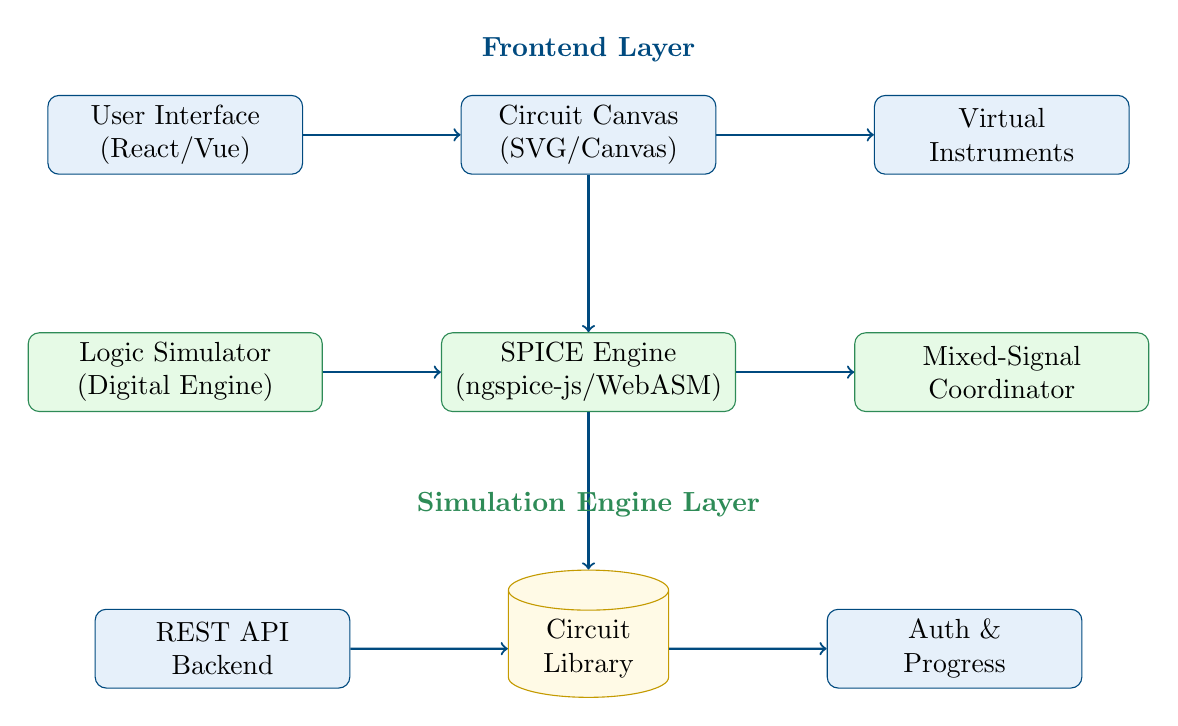
\begin{tikzpicture}[
    node distance=1.5cm,
    block/.style={rectangle, draw=primaryblue, fill=lightblue, text width=3cm, text centered, minimum height=1cm, rounded corners},
    engine/.style={rectangle, draw=successgreen, fill=lightgreen, text width=3.5cm, text centered, minimum height=1cm, rounded corners},
    storage/.style={cylinder, draw=accentgold, fill=lightyellow, shape border rotate=90, aspect=0.25, minimum height=1.2cm, minimum width=2cm, text width=1.8cm, align=center},
    arrow/.style={->, thick, primaryblue}
]

% Frontend Layer
\node[block] (ui) {User Interface\\(React/Vue)};
\node[block, right=2cm of ui] (canvas) {Circuit Canvas\\(SVG/Canvas)};
\node[block, right=2cm of canvas] (tools) {Virtual\\Instruments};

% Simulation Layer
\node[engine, below=2cm of canvas] (spice) {SPICE Engine\\(ngspice-js/WebASM)};
\node[engine, left=1.5cm of spice] (logic) {Logic Simulator\\(Digital Engine)};
\node[engine, right=1.5cm of spice] (mixed) {Mixed-Signal\\Coordinator};

% Backend/Storage Layer
\node[storage, below=2cm of spice] (circuits) {Circuit\\Library};
\node[block, left=2cm of circuits] (api) {REST API\\Backend};
\node[block, right=2cm of circuits] (auth) {Auth \&\\Progress};

% Arrows
\draw[arrow] (ui) -- (canvas);
\draw[arrow] (canvas) -- (tools);
\draw[arrow] (canvas) -- (spice);
\draw[arrow] (logic) -- (spice);
\draw[arrow] (spice) -- (mixed);
\draw[arrow] (spice) -- (circuits);
\draw[arrow] (api) -- (circuits);
\draw[arrow] (circuits) -- (auth);

% Labels
\node[above=0.3cm of canvas, color=primaryblue, font=\bfseries] {Frontend Layer};
\node[below=0.1cm of spice, yshift=-0.8cm, color=successgreen, font=\bfseries] {Simulation Engine Layer};

\end{tikzpicture}
\caption{High-Level System Architecture}
\label{fig:architecture}
\end{figure}

\section{Simulation Engine Requirements}

\begin{techbox}
The simulation engine must support the following capabilities:

\textbf{Analog Simulation (SPICE-based):}
\begin{itemize}[leftmargin=*, nosep]
    \item DC operating point analysis
    \item AC frequency response (Bode plots)
    \item Transient analysis with configurable time steps
    \item Noise analysis (thermal, shot, 1/f)
    \item Parameter sweeps and Monte Carlo analysis
    \item Support for standard component models (resistors, capacitors, inductors, diodes, BJTs, MOSFETs, op-amps)
\end{itemize}

\textbf{Digital Simulation:}
\begin{itemize}[leftmargin=*, nosep]
    \item Gate-level logic simulation
    \item Propagation delay modeling
    \item Setup/hold time checking
    \item State machine visualization
    \item Bus timing analysis
\end{itemize}

\textbf{Mixed-Signal:}
\begin{itemize}[leftmargin=*, nosep]
    \item ADC/DAC behavioral models
    \item Sample-and-hold dynamics
    \item Quantization noise representation
    \item Clock domain interactions
\end{itemize}
\end{techbox}

\section{Technology Stack Recommendations}

\subsection{Frontend Technologies}

\begin{table}[H]
\centering
\caption{Recommended Frontend Stack}
\begin{tabularx}{\textwidth}{@{}llX@{}}
\toprule
\textbf{Component} & \textbf{Technology} & \textbf{Rationale} \\
\midrule
UI Framework & React 18+ or Vue 3 & Component-based architecture, large ecosystem \\
State Management & Redux Toolkit / Pinia & Complex simulation state handling \\
Circuit Rendering & SVG + D3.js & Vector graphics for schematic display \\
Waveform Display & Chart.js / Plotly.js & High-performance time-domain plotting \\
Canvas Operations & Fabric.js / Konva.js & Interactive schematic manipulation \\
Build System & Vite & Fast development builds, ESM native \\
\bottomrule
\end{tabularx}
\end{table}

\subsection{Simulation Engine Options}

\begin{table}[H]
\centering
\caption{Simulation Engine Comparison}
\begin{tabularx}{\textwidth}{@{}lXXl@{}}
\toprule
\textbf{Engine} & \textbf{Advantages} & \textbf{Disadvantages} & \textbf{Use Case} \\
\midrule
ngspice (WebAssembly) & Full SPICE accuracy, extensive model library & Large binary size ($\sim$5MB), complex integration & Primary analog engine \\
\addlinespace
CircuitJS & Lightweight, educational focus, open source & Limited accuracy for precision circuits & Quick demonstrations \\
\addlinespace
Custom TypeScript & Full control, optimized for web & Development effort, limited models & Digital logic, simple analog \\
\addlinespace
Server-side SPICE & Maximum accuracy, all features & Latency, server costs, scaling challenges & Precision verification \\
\bottomrule
\end{tabularx}
\end{table}

\subsection{Recommended Hybrid Approach}

\begin{enumerate}[leftmargin=*, itemsep=4pt]
    \item \textbf{Client-Side Primary:} Use WebAssembly-compiled ngspice for most analog simulations, running entirely in the browser for responsiveness.
    
    \item \textbf{Custom Digital Engine:} Implement a purpose-built TypeScript logic simulator for digital circuits, optimized for the specific needs of the curriculum.
    
    \item \textbf{Server-Side Fallback:} Provide server-based simulation for complex circuits (noise analysis, Monte Carlo) where accuracy is paramount.
    
    \item \textbf{Progressive Enhancement:} Start with simpler simulations and progressively add complexity based on user hardware capabilities.
\end{enumerate}

\subsection{Backend Technologies}

\begin{table}[H]
\centering
\caption{Recommended Backend Stack}
\begin{tabularx}{\textwidth}{@{}llX@{}}
\toprule
\textbf{Component} & \textbf{Technology} & \textbf{Rationale} \\
\midrule
API Server & Node.js/Express or Python/FastAPI & REST API, WebSocket for real-time \\
Database & PostgreSQL + Redis & Relational data + caching \\
Authentication & Auth0 / Firebase Auth & Managed auth, social login \\
File Storage & AWS S3 / Cloudflare R2 & Circuit files, user projects \\
Server SPICE & ngspice containerized & Accurate simulation fallback \\
Deployment & Vercel / AWS / GCP & Scalable hosting \\
\bottomrule
\end{tabularx}
\end{table}

\section{Data Models}

\subsection{Circuit Definition Schema}

Circuits will be defined using a JSON-based schema that captures both schematic and simulation parameters:

\begin{verbatim}
{
  "id": "phase1_opamp_inverting",
  "name": "Inverting Op-Amp Amplifier",
  "curriculum": {
    "source": "aoe_main",
    "phase": 1,
    "section": "1.3.2",
    "aoe_reference": "Chapter 4, Section 4.2"
  },
  "components": [
    {"type": "opamp", "id": "U1", "model": "TL072", ...},
    {"type": "resistor", "id": "R1", "value": "10k", ...}
  ],
  "connections": [...],
  "simulation": {
    "analyses": ["dc", "ac", "transient"],
    "default_params": {...}
  },
  "exercises": [...]
}
\end{verbatim}

\clearpage

% ============================================================================
% CHAPTER 3: CIRCUIT INVENTORY - AOE MAIN CURRICULUM
% ============================================================================
\chapter{Circuit Inventory: AoE Main Curriculum}
\label{ch:aoe_circuits}

This chapter provides a comprehensive inventory of all circuits from the main \aoe{} laboratory curriculum that must be implemented in the simulator.

\section{Phase 0: Orientation \& Laboratory Setup}

\begin{phasebox}[phase1color]{Phase 0 Circuits --- Foundation \& Measurement}

\textbf{Duration:} 1--2 weeks \hfill \textbf{Circuit Count:} 8 circuits

This phase establishes measurement fundamentals and basic circuit behavior verification.
\end{phasebox}

\begin{circuitbox}[Phase 0 Circuit List]
\begin{enumerate}[leftmargin=*, itemsep=4pt]
    \item \textbf{7805 Linear Voltage Regulator}
    \begin{itemize}[nosep]
        \item Basic 12V to 5V regulation with input/output capacitors
        \item Simulations: Line regulation, load regulation, ripple rejection, thermal behavior
        \item Measurements: $V_{out}$ vs $V_{in}$, $V_{out}$ vs $I_{load}$, dropout voltage
    \end{itemize}
    
    \item \textbf{RC Low-Pass Filter (First-Order)}
    \begin{itemize}[nosep]
        \item Simple RC network for frequency response fundamentals
        \item Simulations: Bode plot (magnitude/phase), step response, square wave response
        \item Cutoff frequency calculation and verification
    \end{itemize}
    
    \item \textbf{RC High-Pass Filter (First-Order)}
    \begin{itemize}[nosep]
        \item Complementary to low-pass for complete filter understanding
        \item AC coupling behavior demonstration
    \end{itemize}
    
    \item \textbf{Voltage Divider Networks}
    \begin{itemize}[nosep]
        \item Basic resistive dividers with loading effects
        \item Source impedance and load impedance interactions
    \end{itemize}
    
    \item \textbf{Diode Rectifier (Half-Wave)}
    \begin{itemize}[nosep]
        \item Basic rectification with 1N400x diodes
        \item Peak detection, ripple analysis
    \end{itemize}
    
    \item \textbf{Diode Rectifier (Full-Wave Bridge)}
    \begin{itemize}[nosep]
        \item Bridge rectifier with filter capacitor
        \item Ripple voltage calculation, capacitor sizing
    \end{itemize}
    
    \item \textbf{Zener Diode Regulator}
    \begin{itemize}[nosep]
        \item Simple shunt regulation
        \item Line and load regulation characteristics
    \end{itemize}
    
    \item \textbf{LED Current Limiting}
    \begin{itemize}[nosep]
        \item Basic LED driver with series resistor
        \item Forward voltage drop, current calculation
    \end{itemize}
\end{enumerate}
\end{circuitbox}

\section{Phase 1: Analog Foundations \& Building Blocks}

\begin{phasebox}[phase1color]{Phase 1 Circuits --- Analog Core}

\textbf{Duration:} 3--4 weeks \hfill \textbf{Circuit Count:} 25 circuits

Core analog building blocks including op-amp configurations, filters, and transistor circuits.
\end{phasebox}

\subsection{Op-Amp Configurations}

\begin{circuitbox}[Op-Amp Circuits]
\begin{enumerate}[leftmargin=*, itemsep=4pt]
    \item \textbf{Inverting Amplifier}
    \begin{itemize}[nosep]
        \item Configurable gain (1, 10, 100)
        \item Virtual ground concept demonstration
        \item Simulations: DC gain, bandwidth, slew rate, input/output impedance
    \end{itemize}
    
    \item \textbf{Non-Inverting Amplifier}
    \begin{itemize}[nosep]
        \item High input impedance configuration
        \item Gain-bandwidth product demonstration
    \end{itemize}
    
    \item \textbf{Unity-Gain Buffer (Voltage Follower)}
    \begin{itemize}[nosep]
        \item Impedance transformation
        \item Loading effect elimination
    \end{itemize}
    
    \item \textbf{Summing Amplifier}
    \begin{itemize}[nosep]
        \item Multiple input weighted summation
        \item Audio mixer application
    \end{itemize}
    
    \item \textbf{Difference Amplifier}
    \begin{itemize}[nosep]
        \item Basic differential measurement
        \item CMRR demonstration
    \end{itemize}
    
    \item \textbf{Integrator}
    \begin{itemize}[nosep]
        \item Op-amp with capacitive feedback
        \item Square-to-triangle conversion
        \item DC offset management
    \end{itemize}
    
    \item \textbf{Differentiator}
    \begin{itemize}[nosep]
        \item High-frequency noise amplification issue
        \item Practical differentiator with limiting resistor
    \end{itemize}
    
    \item \textbf{Comparator}
    \begin{itemize}[nosep]
        \item Open-loop op-amp operation
        \item Hysteresis (Schmitt trigger) addition
    \end{itemize}
\end{enumerate}
\end{circuitbox}

\subsection{Active Filters}

\begin{circuitbox}[Active Filter Circuits]
\begin{enumerate}[leftmargin=*, itemsep=4pt]
    \item \textbf{Sallen-Key Low-Pass Filter (2nd Order)}
    \begin{itemize}[nosep]
        \item Butterworth response (Q = 0.707)
        \item Selectable cutoff: 1kHz, 10kHz
        \item 40 dB/decade rolloff demonstration
    \end{itemize}
    
    \item \textbf{Sallen-Key High-Pass Filter (2nd Order)}
    \begin{itemize}[nosep]
        \item Complementary high-pass design
        \item Audio applications (DC blocking)
    \end{itemize}
    
    \item \textbf{Multiple Feedback (MFB) Bandpass Filter}
    \begin{itemize}[nosep]
        \item Center frequency and Q selection
        \item Audio tone detection
    \end{itemize}
    
    \item \textbf{State-Variable Filter}
    \begin{itemize}[nosep]
        \item Simultaneous LP, HP, BP outputs
        \item Independent Q and frequency control
    \end{itemize}
    
    \item \textbf{Twin-T Notch Filter}
    \begin{itemize}[nosep]
        \item 50/60 Hz hum rejection
        \item Deep null at target frequency
    \end{itemize}
\end{enumerate}
\end{circuitbox}

\subsection{Transistor Circuits}

\begin{circuitbox}[Transistor Circuits]
\begin{enumerate}[leftmargin=*, itemsep=4pt]
    \item \textbf{BJT Switch (NPN)}
    \begin{itemize}[nosep]
        \item 2N3904/2N2222 saturation switching
        \item Base resistor calculation for hard saturation
        \item LED driver, relay driver applications
    \end{itemize}
    
    \item \textbf{BJT Switch (PNP)}
    \begin{itemize}[nosep]
        \item High-side switching configuration
        \item Complementary to NPN designs
    \end{itemize}
    
    \item \textbf{MOSFET Switch (N-Channel)}
    \begin{itemize}[nosep]
        \item 2N7000/BS170 logic-level switching
        \item Gate threshold and $R_{DS(on)}$ demonstration
    \end{itemize}
    
    \item \textbf{Emitter Follower (Common Collector)}
    \begin{itemize}[nosep]
        \item Unity voltage gain buffer
        \item High input impedance, low output impedance
        \item Current gain demonstration
    \end{itemize}
    
    \item \textbf{Source Follower (Common Drain)}
    \begin{itemize}[nosep]
        \item JFET-based high-impedance buffer
        \item Very high input impedance ($>10^{12}\Omega$)
    \end{itemize}
    
    \item \textbf{Common Emitter Amplifier}
    \begin{itemize}[nosep]
        \item Basic voltage amplifier stage
        \item Biasing, gain, bandwidth trade-offs
    \end{itemize}
    
    \item \textbf{Darlington Pair}
    \begin{itemize}[nosep]
        \item High current gain ($\beta^2$)
        \item Buffer applications
    \end{itemize}
    
    \item \textbf{Current Mirror}
    \begin{itemize}[nosep]
        \item Basic BJT current mirror
        \item Wilson and Widlar variations
    \end{itemize}
\end{enumerate}
\end{circuitbox}

\section{Phase 2: Precision \& Low-Noise Instrumentation}

\begin{phasebox}[phase2color]{Phase 2 Circuits --- Precision \& Noise}

\textbf{Duration:} 4--5 weeks \hfill \textbf{Circuit Count:} 18 circuits

Precision measurement circuits with noise analysis capabilities.
\end{phasebox}

\begin{circuitbox}[Precision Circuits]
\begin{enumerate}[leftmargin=*, itemsep=4pt]
    \item \textbf{Three-Op-Amp Instrumentation Amplifier}
    \begin{itemize}[nosep]
        \item High CMRR ($>$100 dB) differential amplifier
        \item Single resistor gain setting
        \item Bridge sensor interface (strain gauge, load cell)
    \end{itemize}
    
    \item \textbf{Integrated Instrumentation Amplifier (INA128/AD620)}
    \begin{itemize}[nosep]
        \item Commercial in-amp behavior modeling
        \item CMRR vs frequency, gain accuracy
    \end{itemize}
    
    \item \textbf{Transimpedance Amplifier (Photodiode Front-End)}
    \begin{itemize}[nosep]
        \item Current-to-voltage conversion
        \item Photodiode capacitance compensation
        \item Noise analysis: voltage noise, current noise, thermal noise
    \end{itemize}
    
    \item \textbf{Low-Noise Preamplifier}
    \begin{itemize}[nosep]
        \item Optimized for minimum noise figure
        \item Input-referred noise calculation
    \end{itemize}
    
    \item \textbf{Chopper-Stabilized Amplifier}
    \begin{itemize}[nosep]
        \item Auto-zero offset cancellation
        \item 1/f noise elimination
    \end{itemize}
    
    \item \textbf{Precision Voltage Reference}
    \begin{itemize}[nosep]
        \item Bandgap reference behavior (REF5050, LM4040)
        \item Temperature coefficient, load regulation
    \end{itemize}
    
    \item \textbf{Kelvin (4-Wire) Resistance Measurement}
    \begin{itemize}[nosep]
        \item Lead resistance elimination
        \item RTD temperature sensing
    \end{itemize}
    
    \item \textbf{Wheatstone Bridge}
    \begin{itemize}[nosep]
        \item Bridge excitation and balance
        \item Strain gauge signal conditioning
    \end{itemize}
    
    \item \textbf{Active Guard Driver}
    \begin{itemize}[nosep]
        \item Leakage current elimination
        \item High-impedance node protection
    \end{itemize}
    
    \item \textbf{Sample-and-Hold Circuit}
    \begin{itemize}[nosep]
        \item Acquisition time, droop rate
        \item ADC front-end application
    \end{itemize}
\end{enumerate}
\end{circuitbox}

\subsection{Noise Analysis Features}

The Phase 2 simulations must include comprehensive noise analysis capabilities:

\begin{itemize}[leftmargin=*, itemsep=4pt]
    \item \textbf{Noise Spectral Density:} Display $\si{\nano\volt/\sqrt{Hz}}$ or $\si{\pico\ampere/\sqrt{Hz}}$ vs frequency
    \item \textbf{Integrated Noise:} Calculate RMS noise over specified bandwidth
    \item \textbf{Noise Budget Tool:} Interactive calculator showing contributions from each component
    \item \textbf{1/f Corner Frequency:} Identification of flicker noise corner
    \item \textbf{Signal-to-Noise Ratio:} SNR calculation for given signal levels
\end{itemize}

\section{Phase 3: Power Electronics \& Protection}

\begin{phasebox}[phase3color]{Phase 3 Circuits --- Power}

\textbf{Duration:} 4--5 weeks \hfill \textbf{Circuit Count:} 15 circuits

Power supply design, switching regulators, and protection circuits.
\end{phasebox}

\begin{circuitbox}[Power Supply Circuits]
\begin{enumerate}[leftmargin=*, itemsep=4pt]
    \item \textbf{LM317 Adjustable Regulator}
    \begin{itemize}[nosep]
        \item Adjustable output voltage design
        \item Current limiting, thermal protection
    \end{itemize}
    
    \item \textbf{Discrete Linear Regulator (Pass Transistor)}
    \begin{itemize}[nosep]
        \item Op-amp + pass transistor topology
        \item Feedback loop compensation
        \item Foldback current limiting
    \end{itemize}
    
    \item \textbf{Buck Converter (Step-Down)}
    \begin{itemize}[nosep]
        \item Basic switching topology
        \item Inductor sizing, ripple calculation
        \item Continuous vs discontinuous conduction
    \end{itemize}
    
    \item \textbf{Boost Converter (Step-Up)}
    \begin{itemize}[nosep]
        \item Voltage step-up from lower input
        \item Duty cycle vs output voltage relationship
    \end{itemize}
    
    \item \textbf{Buck-Boost Converter}
    \begin{itemize}[nosep]
        \item Inverting topology
        \item Input voltage range flexibility
    \end{itemize}
    
    \item \textbf{Synchronous Buck Converter}
    \begin{itemize}[nosep]
        \item High-efficiency design with active rectification
        \item Dead-time control, shoot-through prevention
    \end{itemize}
    
    \item \textbf{Flyback Converter}
    \begin{itemize}[nosep]
        \item Isolated power supply topology
        \item Transformer design considerations
    \end{itemize}
    
    \item \textbf{Current Limiting Circuit}
    \begin{itemize}[nosep]
        \item Constant current, foldback limiting
        \item Pass device protection
    \end{itemize}
    
    \item \textbf{Crowbar Overvoltage Protection}
    \begin{itemize}[nosep]
        \item SCR-based protection
        \item Fuse coordination
    \end{itemize}
    
    \item \textbf{Soft-Start Circuit}
    \begin{itemize}[nosep]
        \item Inrush current limiting
        \item Capacitor-controlled ramp
    \end{itemize}
    
    \item \textbf{Reverse Polarity Protection}
    \begin{itemize}[nosep]
        \item Diode vs P-FET protection
        \item Voltage drop considerations
    \end{itemize}
\end{enumerate}
\end{circuitbox}

\section{Phase 4: Digital Logic \& Mixed-Signal}

\begin{phasebox}[phase4color]{Phase 4 Circuits --- Digital \& Mixed}

\textbf{Duration:} 4--5 weeks \hfill \textbf{Circuit Count:} 20 circuits

Digital logic, data conversion, and mixed-signal integration.
\end{phasebox}

\begin{circuitbox}[Digital \& Mixed-Signal Circuits]
\begin{enumerate}[leftmargin=*, itemsep=4pt]
    \item \textbf{Level Shifter (5V to 3.3V)}
    \begin{itemize}[nosep]
        \item Resistor divider, dedicated IC approaches
        \item Bidirectional level shifting
    \end{itemize}
    
    \item \textbf{Logic Gate Fundamentals}
    \begin{itemize}[nosep]
        \item AND, OR, NAND, NOR, XOR gates
        \item Propagation delay, fan-out
    \end{itemize}
    
    \item \textbf{D Flip-Flop}
    \begin{itemize}[nosep]
        \item Setup/hold time demonstration
        \item Metastability visualization
    \end{itemize}
    
    \item \textbf{Binary Counter}
    \begin{itemize}[nosep]
        \item Ripple vs synchronous
        \item Timing analysis
    \end{itemize}
    
    \item \textbf{Shift Register}
    \begin{itemize}[nosep]
        \item Serial-to-parallel conversion
        \item SPI interface fundamentals
    \end{itemize}
    
    \item \textbf{R-2R DAC}
    \begin{itemize}[nosep]
        \item Basic digital-to-analog conversion
        \item Monotonicity, DNL, INL
    \end{itemize}
    
    \item \textbf{Flash ADC (3-bit)}
    \begin{itemize}[nosep]
        \item Parallel comparator architecture
        \item Speed vs resolution trade-off
    \end{itemize}
    
    \item \textbf{Successive Approximation ADC}
    \begin{itemize}[nosep]
        \item SAR algorithm visualization
        \item Conversion timing
    \end{itemize}
    
    \item \textbf{Delta-Sigma Modulator}
    \begin{itemize}[nosep]
        \item Oversampling concept
        \item Noise shaping demonstration
    \end{itemize}
    
    \item \textbf{Anti-Aliasing Filter}
    \begin{itemize}[nosep]
        \item Nyquist frequency considerations
        \item Filter order vs aliasing
    \end{itemize}
    
    \item \textbf{PWM Generation}
    \begin{itemize}[nosep]
        \item Timer-based PWM
        \item Analog reconstruction
    \end{itemize}
    
    \item \textbf{Button Debouncing}
    \begin{itemize}[nosep]
        \item Hardware RC debounce
        \item Software debounce algorithm
    \end{itemize}
    
    \item \textbf{I2C Interface}
    \begin{itemize}[nosep]
        \item Pull-up resistor selection
        \item Bus timing, clock stretching
    \end{itemize}
    
    \item \textbf{SPI Interface}
    \begin{itemize}[nosep]
        \item Clock polarity/phase modes
        \item Multi-device bus
    \end{itemize}
\end{enumerate}
\end{circuitbox}

\section{Phase 5: High-Speed \& RF-Lite}

\begin{phasebox}[phase5color]{Phase 5 Circuits --- High-Speed}

\textbf{Duration:} 4--6 weeks \hfill \textbf{Circuit Count:} 12 circuits

High-frequency design, transmission lines, and signal integrity.
\end{phasebox}

\begin{circuitbox}[High-Speed Circuits]
\begin{enumerate}[leftmargin=*, itemsep=4pt]
    \item \textbf{Transmission Line (50$\Omega$)}
    \begin{itemize}[nosep]
        \item Reflection visualization with various terminations
        \item Open, short, matched, and mismatched loads
        \item TDR-style analysis
    \end{itemize}
    
    \item \textbf{50$\Omega$ Line Driver}
    \begin{itemize}[nosep]
        \item High-speed buffer design
        \item Output impedance matching
    \end{itemize}
    
    \item \textbf{Current-Feedback Amplifier}
    \begin{itemize}[nosep]
        \item CFB vs VFB comparison
        \item Bandwidth independence from gain
    \end{itemize}
    
    \item \textbf{Video Buffer}
    \begin{itemize}[nosep]
        \item Wide bandwidth, low distortion
        \item Back-termination techniques
    \end{itemize}
    
    \item \textbf{Crystal Oscillator}
    \begin{itemize}[nosep]
        \item Pierce oscillator topology
        \item Load capacitance selection
        \item Start-up behavior
    \end{itemize}
    
    \item \textbf{Phase-Locked Loop (Basic)}
    \begin{itemize}[nosep]
        \item Phase detector, loop filter, VCO
        \item Lock acquisition visualization
    \end{itemize}
    
    \item \textbf{RF Amplifier (Low-Noise)}
    \begin{itemize}[nosep]
        \item Input/output matching
        \item Noise figure optimization
    \end{itemize}
\end{enumerate}
\end{circuitbox}

\clearpage

% ============================================================================
% CHAPTER 4: CIRCUIT INVENTORY - X CHAPTERS
% ============================================================================
\chapter{Circuit Inventory: X Chapters Curriculum}
\label{ch:xchapters_circuits}

The X Chapters curriculum represents advanced topics requiring sophisticated simulation capabilities.

\section{Phase 1: Advanced Analog \& Power Core}

\subsection{Project A1: Multi-Output Lab Power Supply}

\begin{circuitbox}[A1 Power Supply Circuits]
Complete multi-rail laboratory power supply with the following subsystems:

\begin{enumerate}[leftmargin=*, itemsep=4pt]
    \item \textbf{5V/3A Digital Rail}
    \begin{itemize}[nosep]
        \item Fixed output with tight regulation
        \item Overcurrent protection
    \end{itemize}
    
    \item \textbf{3.3V/3A Digital Rail}
    \begin{itemize}[nosep]
        \item Modern logic/MCU supply
        \item Low-noise design for sensitive digital
    \end{itemize}
    
    \item \textbf{Adjustable 0--24V/3A Rail}
    \begin{itemize}[nosep]
        \item Wide output range with constant regulation
        \item Pre-regulator + linear post-regulator topology
        \item Foldback current limiting visualization
    \end{itemize}
    
    \item \textbf{$\pm$12V/1A Symmetric Rails}
    \begin{itemize}[nosep]
        \item Op-amp supply rails
        \item Tracking behavior demonstration
        \item Start-up sequencing
    \end{itemize}
    
    \item \textbf{Protection Circuits}
    \begin{itemize}[nosep]
        \item SOA (Safe Operating Area) visualization
        \item Thermal shutdown modeling
        \item Reverse current protection
    \end{itemize}
    
    \item \textbf{Loop Compensation}
    \begin{itemize}[nosep]
        \item Bode plot analysis
        \item Phase margin, gain margin visualization
        \item Step load transient response
    \end{itemize}
\end{enumerate}
\end{circuitbox}

\subsection{Project A2: Precision Transresistance Amplifier}

\begin{circuitbox}[A2 TIA Circuits]
Low-noise photodiode amplifier with femtoampere sensitivity:

\begin{enumerate}[leftmargin=*, itemsep=4pt]
    \item \textbf{Ultra-Low-Noise TIA (Slow)}
    \begin{itemize}[nosep]
        \item Bandwidth: 1--10 kHz
        \item Input-referred noise: $<$10 fA/$\sqrt{\text{Hz}}$
        \item FET-input op-amp (OPA627, AD549)
    \end{itemize}
    
    \item \textbf{Fast TIA}
    \begin{itemize}[nosep]
        \item Bandwidth: 100 kHz -- 1 MHz
        \item Noise-bandwidth trade-off demonstration
    \end{itemize}
    
    \item \textbf{Noise Analysis Features}
    \begin{itemize}[nosep]
        \item Johnson-Nyquist noise visualization
        \item Op-amp voltage/current noise
        \item Noise bandwidth calculation
    \end{itemize}
    
    \item \textbf{Stability Compensation}
    \begin{itemize}[nosep]
        \item Photodiode capacitance effect
        \item Feedback capacitor sizing
        \item Phase margin optimization
    \end{itemize}
\end{enumerate}
\end{circuitbox}

\subsection{Project A3: High-Speed Op-Amp Circuit}

\begin{circuitbox}[A3 High-Speed Circuits]
High-frequency amplifier designs (50+ MHz bandwidth):

\begin{enumerate}[leftmargin=*, itemsep=4pt]
    \item \textbf{Gain-of-10 VFB Amplifier}
    \begin{itemize}[nosep]
        \item Voltage-feedback topology
        \item GBW product verification
    \end{itemize}
    
    \item \textbf{Gain-of-10 CFB Amplifier}
    \begin{itemize}[nosep]
        \item Current-feedback topology comparison
        \item Bandwidth vs gain behavior
    \end{itemize}
    
    \item \textbf{Differential Amplifier}
    \begin{itemize}[nosep]
        \item Single-ended to differential conversion
        \item Matched delay paths
    \end{itemize}
    
    \item \textbf{PCB Parasitic Effects}
    \begin{itemize}[nosep]
        \item Trace inductance modeling
        \item Ground plane effects
        \item Decoupling effectiveness
    \end{itemize}
\end{enumerate}
\end{circuitbox}

\subsection{Project A4: High-Energy Pulser / Coil Driver}

\begin{circuitbox}[A4 Power Switching Circuits]
High-current switching circuits with protection:

\begin{enumerate}[leftmargin=*, itemsep=4pt]
    \item \textbf{Fast LED Driver}
    \begin{itemize}[nosep]
        \item Nanosecond pulse generation
        \item 10A peak current capability
    \end{itemize}
    
    \item \textbf{Inductive Coil Driver}
    \begin{itemize}[nosep]
        \item Solenoid actuation
        \item Flyback voltage demonstration
    \end{itemize}
    
    \item \textbf{MOSFET Gate Drive}
    \begin{itemize}[nosep]
        \item Gate charge calculation
        \item Miller plateau visualization
        \item Gate driver IC behavior
    \end{itemize}
    
    \item \textbf{Snubber Design}
    \begin{itemize}[nosep]
        \item RC snubber optimization
        \item RCD clamp circuits
        \item dV/dt and dI/dt control
    \end{itemize}
    
    \item \textbf{Inductive Kickback}
    \begin{itemize}[nosep]
        \item $V = L \cdot di/dt$ visualization
        \item Clamp diode operation
        \item Energy dissipation
    \end{itemize}
\end{enumerate}
\end{circuitbox}

\subsection{Project A5: Precision Measurement Instrument}

\begin{circuitbox}[A5 Measurement Circuits]
Complete measurement front-end integration:

\begin{enumerate}[leftmargin=*, itemsep=4pt]
    \item \textbf{Precision DC Voltmeter Front-End}
    \begin{itemize}[nosep]
        \item $\pm$10$\mu$V to $\pm$10V range
        \item Input impedance $>$1G$\Omega$
        \item 1$\mu$V resolution
    \end{itemize}
    
    \item \textbf{Low-Noise AC Probe}
    \begin{itemize}[nosep]
        \item 1 Hz -- 100 kHz bandwidth
        \item $<$10 nV/$\sqrt{\text{Hz}}$ noise floor
        \item Differential input, high CMRR
    \end{itemize}
    
    \item \textbf{Simple Impedance Probe}
    \begin{itemize}[nosep]
        \item R, L, C measurement at fixed frequencies
        \item Phase detection
        \item Component verification
    \end{itemize}
    
    \item \textbf{Error Budget Analysis}
    \begin{itemize}[nosep]
        \item Interactive error source tracking
        \item Offset, gain, linearity errors
        \item Temperature coefficient effects
    \end{itemize}
\end{enumerate}
\end{circuitbox}

\section{Phase 2: Digital \& Embedded Foundations}

\subsection{Project D1: Breadboard Computer}

\begin{circuitbox}[D1 CPU Building Blocks]
Discrete logic implementation of a minimal processor:

\begin{enumerate}[leftmargin=*, itemsep=4pt]
    \item \textbf{Clock Generator}
    \begin{itemize}[nosep]
        \item Crystal oscillator or 555-based
        \item Single-step mode for debugging
    \end{itemize}
    
    \item \textbf{Program Counter}
    \begin{itemize}[nosep]
        \item 8-bit counter with load capability
        \item Jump instruction support
    \end{itemize}
    
    \item \textbf{Register File}
    \begin{itemize}[nosep]
        \item 4--8 general-purpose registers
        \item Read/write port timing
    \end{itemize}
    
    \item \textbf{ALU (Arithmetic Logic Unit)}
    \begin{itemize}[nosep]
        \item ADD, AND, OR, XOR operations
        \item Carry/overflow flag generation
    \end{itemize}
    
    \item \textbf{Instruction Decoder}
    \begin{itemize}[nosep]
        \item ROM-based microcode or hardwired
        \item Control signal generation
    \end{itemize}
    
    \item \textbf{Memory Interface}
    \begin{itemize}[nosep]
        \item Address decoding
        \item Read/write cycle timing
        \item Memory-mapped I/O
    \end{itemize}
    
    \item \textbf{Bus Architecture}
    \begin{itemize}[nosep]
        \item Tristate buffer control
        \item Bus contention detection
    \end{itemize}
\end{enumerate}
\end{circuitbox}

\subsection{Project D2: FPGA-Based System}

\begin{circuitbox}[D2 FPGA Circuits]
HDL-based digital system with analog interfaces:

\begin{enumerate}[leftmargin=*, itemsep=4pt]
    \item \textbf{Simple Processor Core}
    \begin{itemize}[nosep]
        \item Behavioral simulation of instruction execution
        \item Register transfer level visualization
    \end{itemize}
    
    \item \textbf{SPI Master Controller}
    \begin{itemize}[nosep]
        \item Configurable clock rate
        \item Multiple device support
    \end{itemize}
    
    \item \textbf{UART Transmitter/Receiver}
    \begin{itemize}[nosep]
        \item Baud rate generation
        \item Start/stop bit framing
    \end{itemize}
    
    \item \textbf{PWM Controller}
    \begin{itemize}[nosep]
        \item Variable frequency and duty cycle
        \item Dead-time insertion
    \end{itemize}
    
    \item \textbf{ADC Interface}
    \begin{itemize}[nosep]
        \item SPI-based ADC control
        \item Sample timing coordination
    \end{itemize}
    
    \item \textbf{Clock Domain Crossing}
    \begin{itemize}[nosep]
        \item Two-flip-flop synchronizer
        \item Gray code counter crossing
        \item Async FIFO
    \end{itemize}
\end{enumerate}
\end{circuitbox}

\section{Phase 3: Embedded Systems with RTOS}

\subsection{Project E1: ARM MCU + RTOS Platform}

\begin{circuitbox}[E1 Embedded Circuits]
MCU peripheral interface circuits:

\begin{enumerate}[leftmargin=*, itemsep=4pt]
    \item \textbf{MCU Power Supply Filtering}
    \begin{itemize}[nosep]
        \item Decoupling capacitor placement
        \item Ferrite bead usage
    \end{itemize}
    
    \item \textbf{Crystal Oscillator Interface}
    \begin{itemize}[nosep]
        \item Load capacitor selection
        \item Start-up reliability
    \end{itemize}
    
    \item \textbf{Reset Circuit}
    \begin{itemize}[nosep]
        \item Brown-out detection
        \item Manual reset debouncing
    \end{itemize}
    
    \item \textbf{Debug Interface (SWD)}
    \begin{itemize}[nosep]
        \item Connector pinout
        \item Series resistor protection
    \end{itemize}
    
    \item \textbf{GPIO Protection}
    \begin{itemize}[nosep]
        \item ESD protection
        \item Current limiting
    \end{itemize}
\end{enumerate}
\end{circuitbox}

\subsection{Project E2: Embedded Instrument / Controller}

\begin{circuitbox}[E2 System Integration Circuits]
Complete system integration simulations:

\begin{enumerate}[leftmargin=*, itemsep=4pt]
    \item \textbf{Digitally-Controlled Power Supply}
    \begin{itemize}[nosep]
        \item DAC/PWM setpoint control
        \item ADC voltage/current monitoring
        \item Closed-loop regulation
    \end{itemize}
    
    \item \textbf{Data Acquisition System}
    \begin{itemize}[nosep]
        \item Multi-channel ADC sampling
        \item Triggering and capture
        \item SD card interface
    \end{itemize}
    
    \item \textbf{Function Generator}
    \begin{itemize}[nosep]
        \item DDS waveform synthesis
        \item DAC reconstruction
        \item Output conditioning
    \end{itemize}
    
    \item \textbf{Mixed-Signal Grounding}
    \begin{itemize}[nosep]
        \item Ground plane partitioning
        \item Star grounding
        \item Digital noise isolation
    \end{itemize}
\end{enumerate}
\end{circuitbox}

\clearpage

% ============================================================================
% CHAPTER 5: USER INTERFACE DESIGN
% ============================================================================
\chapter{User Interface Design}
\label{ch:ui_design}

\section{Core UI Components}

\subsection{Circuit Canvas}

The primary interaction surface for circuit manipulation:

\begin{itemize}[leftmargin=*, itemsep=4pt]
    \item \textbf{Schematic View:} Traditional electronics schematic representation with standard symbols
    \item \textbf{Component Palette:} Drag-and-drop component library organized by category
    \item \textbf{Wire Routing:} Automatic orthogonal routing with manual override capability
    \item \textbf{Node Highlighting:} Visual indication of connected nodes
    \item \textbf{Zoom/Pan:} Smooth navigation for complex circuits
    \item \textbf{Grid Snap:} Configurable grid for neat layouts
\end{itemize}

\subsection{Virtual Instruments}

\begin{table}[H]
\centering
\caption{Virtual Instrument Requirements}
\begin{tabularx}{\textwidth}{@{}lXl@{}}
\toprule
\textbf{Instrument} & \textbf{Features} & \textbf{Priority} \\
\midrule
Digital Multimeter & DC/AC voltage, current, resistance, continuity & P0 \\
Oscilloscope & 2--4 channels, triggering, cursors, FFT, XY mode & P0 \\
Function Generator & Sine, square, triangle, arbitrary waveforms & P0 \\
Bode Plotter & Magnitude/phase vs frequency, log/linear scales & P0 \\
Power Supply & Adjustable voltage/current, display, limiting & P1 \\
Spectrum Analyzer & FFT-based frequency domain display & P1 \\
Logic Analyzer & Multi-channel digital capture, protocol decode & P2 \\
Curve Tracer & I-V characteristic plotting for semiconductors & P2 \\
\bottomrule
\end{tabularx}
\end{table}

\subsection{Simulation Controls}

\begin{itemize}[leftmargin=*, itemsep=4pt]
    \item \textbf{Analysis Selection:} DC operating point, AC sweep, transient, noise
    \item \textbf{Parameter Entry:} Time range, frequency range, sweep points
    \item \textbf{Run Controls:} Start, stop, pause, single-step
    \item \textbf{Progress Indication:} Simulation progress for long analyses
    \item \textbf{Results Management:} Save, load, export simulation data
\end{itemize}

\section{Educational Features}

\subsection{Guided Exercises}

Each circuit includes structured learning activities:

\begin{enumerate}[leftmargin=*, itemsep=4pt]
    \item \textbf{Objective Statement:} Clear learning goal
    \item \textbf{Step-by-Step Instructions:} Guided procedure
    \item \textbf{Measurement Challenges:} Specific values to measure
    \item \textbf{Calculation Verification:} Compare calculated vs simulated
    \item \textbf{``What If'' Explorations:} Guided parameter variations
    \item \textbf{Troubleshooting Scenarios:} Diagnose intentionally faulty circuits
\end{enumerate}

\subsection{AoE Reference Integration}

\begin{itemize}[leftmargin=*, itemsep=4pt]
    \item \textbf{Section Links:} Direct references to AoE book sections
    \item \textbf{Rule-of-Thumb Display:} Relevant rules shown in context
    \item \textbf{Equation Reference:} Key formulas with variable highlighting
    \item \textbf{Design Guidelines:} Practical advice from the text
\end{itemize}

\subsection{Progress Tracking}

\begin{itemize}[leftmargin=*, itemsep=4pt]
    \item \textbf{Curriculum Map:} Visual overview of all phases and circuits
    \item \textbf{Completion Status:} Track completed exercises
    \item \textbf{Achievement Badges:} Gamification elements for motivation
    \item \textbf{Lab Notebook:} Save notes, screenshots, measurement data
\end{itemize}

\section{Responsive Design}

The application must support multiple form factors:

\begin{table}[H]
\centering
\caption{Platform Support Requirements}
\begin{tabularx}{\textwidth}{@{}lXX@{}}
\toprule
\textbf{Platform} & \textbf{Primary Use Case} & \textbf{Constraints} \\
\midrule
Desktop (1920×1080+) & Full simulation environment & None \\
Laptop (1366×768) & Portable learning & Reduced canvas size \\
Tablet (iPad) & Touch-based interaction & No hover states \\
Mobile (phone) & Quick reference, simple circuits & Very limited space \\
\bottomrule
\end{tabularx}
\end{table}

\clearpage

% ============================================================================
% CHAPTER 6: DEVELOPMENT ROADMAP
% ============================================================================
\chapter{Development Roadmap}
\label{ch:roadmap}

\section{Phase I: Foundation (Months 1--5)}

\begin{milestonebox}[Phase I: Core Infrastructure]
\textbf{Goal:} Establish fundamental architecture and demonstrate feasibility with 20 foundational circuits.

\textbf{Deliverables:}
\begin{enumerate}[leftmargin=*, itemsep=4pt]
    \item Core simulation engine integration (ngspice-WebAssembly)
    \item Basic schematic editor with component library
    \item Virtual oscilloscope and multimeter
    \item Phase 0 circuits complete (8 circuits)
    \item Basic op-amp circuits (12 circuits)
    \item User authentication and progress tracking
\end{enumerate}

\textbf{Technical Milestones:}
\begin{itemize}[leftmargin=*, nosep]
    \item Week 4: WebAssembly SPICE engine running in browser
    \item Week 8: Schematic editor MVP with 20 components
    \item Week 12: Oscilloscope displaying transient simulation results
    \item Week 16: First 10 circuits fully functional
    \item Week 20: Phase I complete, internal alpha release
\end{itemize}
\end{milestonebox}

\subsection{Sprint Breakdown: Phase I}

\begin{table}[H]
\centering
\caption{Phase I Sprint Plan}
\begin{tabularx}{\textwidth}{@{}clX@{}}
\toprule
\textbf{Sprint} & \textbf{Duration} & \textbf{Focus} \\
\midrule
1--2 & 4 weeks & Project setup, SPICE engine evaluation and integration \\
3--4 & 4 weeks & Schematic editor core: canvas, components, wiring \\
5--6 & 4 weeks & Simulation pipeline: netlist generation, SPICE execution \\
7--8 & 4 weeks & Virtual instruments: oscilloscope, DMM \\
9--10 & 4 weeks & Circuit library: Phase 0 + basic op-amps \\
\bottomrule
\end{tabularx}
\end{table}

\section{Phase II: Analog Core (Months 6--9)}

\begin{milestonebox}[Phase II: Analog Expansion]
\textbf{Goal:} Complete Phase 1 curriculum circuits and add advanced analysis capabilities.

\textbf{Deliverables:}
\begin{enumerate}[leftmargin=*, itemsep=4pt]
    \item Complete op-amp circuit library (all configurations)
    \item Active filter circuits (Sallen-Key, MFB, state-variable)
    \item Transistor circuits (BJT/MOSFET switches, amplifiers)
    \item Bode plotter for frequency response
    \item AC analysis integration
    \item Parameter sweep functionality
\end{enumerate}

\textbf{Circuit Count:} 25 additional circuits (Total: 45)
\end{milestonebox}

\section{Phase III: Precision \& Power (Months 10--13)}

\begin{milestonebox}[Phase III: Precision \& Power Electronics]
\textbf{Goal:} Add precision instrumentation circuits and power supply simulations.

\textbf{Deliverables:}
\begin{enumerate}[leftmargin=*, itemsep=4pt]
    \item Noise analysis engine and visualization
    \item Instrumentation amplifier circuits
    \item Transimpedance amplifier with noise budget tool
    \item Linear regulator circuits (7805, LM317, discrete)
    \item Switching regulator simulations (buck, boost, buck-boost)
    \item Protection circuit demonstrations
    \item Thermal modeling for power devices
\end{enumerate}

\textbf{Circuit Count:} 33 additional circuits (Total: 78)
\end{milestonebox}

\section{Phase IV: Digital \& Mixed-Signal (Months 14--17)}

\begin{milestonebox}[Phase IV: Digital Integration]
\textbf{Goal:} Add digital logic simulation and mixed-signal capabilities.

\textbf{Deliverables:}
\begin{enumerate}[leftmargin=*, itemsep=4pt]
    \item Digital logic simulation engine
    \item Logic analyzer virtual instrument
    \item ADC/DAC behavioral models
    \item Level shifter and interface circuits
    \item D1 Breadboard Computer simulation
    \item D2 FPGA module simulations
    \item Mixed-signal co-simulation
\end{enumerate}

\textbf{Circuit Count:} 35 additional circuits (Total: 113)
\end{milestonebox}

\section{Phase V: Advanced Topics (Months 18--21)}

\begin{milestonebox}[Phase V: Advanced \& High-Speed]
\textbf{Goal:} Complete X Chapters advanced projects and high-speed simulations.

\textbf{Deliverables:}
\begin{enumerate}[leftmargin=*, itemsep=4pt]
    \item Transmission line simulation with reflections
    \item High-speed amplifier circuits (VFB/CFB)
    \item A1--A5 project complete circuits
    \item E1--E2 embedded system interfaces
    \item PLL and oscillator circuits
    \item RF-lite simulations
\end{enumerate}

\textbf{Circuit Count:} 30 additional circuits (Total: 143)
\end{milestonebox}

\section{Phase VI: Integration \& Polish (Months 22--24)}

\begin{milestonebox}[Phase VI: Production Ready]
\textbf{Goal:} Final integration, polish, and production deployment.

\textbf{Deliverables:}
\begin{enumerate}[leftmargin=*, itemsep=4pt]
    \item Capstone project simulations
    \item Complete curriculum integration
    \item Performance optimization
    \item Mobile responsiveness refinement
    \item Documentation and help system
    \item Production deployment
    \item User feedback integration
\end{enumerate}

\textbf{Final Circuit Count:} 150+ circuits
\end{milestonebox}

\section{Milestone Summary}

\begin{table}[H]
\centering
\caption{Complete Milestone Timeline}
\begin{tabularx}{\textwidth}{@{}lllX@{}}
\toprule
\textbf{Month} & \textbf{Phase} & \textbf{Circuits} & \textbf{Key Milestone} \\
\midrule
5 & I Complete & 20 & Alpha release, core functionality \\
9 & II Complete & 45 & Full analog simulation \\
13 & III Complete & 78 & Precision \& power circuits \\
17 & IV Complete & 113 & Digital \& mixed-signal \\
21 & V Complete & 143 & Advanced topics \\
24 & VI Complete & 150+ & Production launch \\
\bottomrule
\end{tabularx}
\end{table}

\clearpage

% ============================================================================
% CHAPTER 7: RISK ANALYSIS
% ============================================================================
\chapter{Risk Analysis \& Mitigation}
\label{ch:risks}

\section{Technical Risks}

\begin{warningbox}
\textbf{Risk 1: WebAssembly SPICE Performance}

\textbf{Description:} ngspice compiled to WebAssembly may not achieve adequate performance for complex circuits or long transient simulations.

\textbf{Impact:} High --- Core functionality depends on simulation speed.

\textbf{Mitigation Strategies:}
\begin{itemize}[leftmargin=*, nosep]
    \item Implement simulation timeouts with graceful degradation
    \item Offer server-side simulation fallback for complex circuits
    \item Optimize netlists to reduce simulation complexity
    \item Use adaptive time-stepping aggressively
    \item Consider Web Workers for non-blocking simulation
\end{itemize}
\end{warningbox}

\begin{warningbox}
\textbf{Risk 2: Mixed-Signal Simulation Accuracy}

\textbf{Description:} Combining analog SPICE simulation with digital logic simulation while maintaining timing accuracy is challenging.

\textbf{Impact:} Medium --- Affects Phase IV and V circuits.

\textbf{Mitigation Strategies:}
\begin{itemize}[leftmargin=*, nosep]
    \item Use behavioral models for ADC/DAC interfaces
    \item Accept some timing approximation for educational purposes
    \item Document accuracy limitations for users
    \item Implement event-driven digital simulation with analog checkpoints
\end{itemize}
\end{warningbox}

\begin{warningbox}
\textbf{Risk 3: Browser Compatibility}

\textbf{Description:} WebAssembly and advanced JavaScript features may not work consistently across all browsers.

\textbf{Impact:} Medium --- Affects user reach.

\textbf{Mitigation Strategies:}
\begin{itemize}[leftmargin=*, nosep]
    \item Target modern browsers only (Chrome, Firefox, Safari, Edge)
    \item Implement feature detection with clear error messages
    \item Provide system requirements documentation
    \item Test extensively on target platforms
\end{itemize}
\end{warningbox}

\section{Educational Risks}

\begin{warningbox}
\textbf{Risk 4: Simulation vs Reality Gap}

\textbf{Description:} Students may develop unrealistic expectations from simulations that don't capture real-world parasitics, component variations, and environmental factors.

\textbf{Impact:} Medium --- Affects educational effectiveness.

\textbf{Mitigation Strategies:}
\begin{itemize}[leftmargin=*, nosep]
    \item Include explicit ``simulation limitations'' notes with each circuit
    \item Add Monte Carlo analysis for component tolerance
    \item Include parasitic models where significant
    \item Encourage real hardware construction alongside simulation
    \item Document common ``gotchas'' when moving from simulation to hardware
\end{itemize}
\end{warningbox}

\section{Project Risks}

\begin{warningbox}
\textbf{Risk 5: Scope Creep}

\textbf{Description:} The comprehensive nature of the curriculum (150+ circuits) creates risk of never-ending feature additions.

\textbf{Impact:} High --- Affects schedule and budget.

\textbf{Mitigation Strategies:}
\begin{itemize}[leftmargin=*, nosep]
    \item Strict prioritization with P0/P1/P2 classification
    \item Time-boxed phases with hard deadlines
    \item MVP mindset: functional before perfect
    \item Regular scope reviews with stakeholders
    \item ``Version 2'' parking lot for future features
\end{itemize}
\end{warningbox}

\clearpage

% ============================================================================
% CHAPTER 8: TESTING STRATEGY
% ============================================================================
\chapter{Testing \& Validation Strategy}
\label{ch:testing}

\section{Simulation Accuracy Validation}

\subsection{Reference Comparison}

All circuit simulations must be validated against desktop SPICE results:

\begin{enumerate}[leftmargin=*, itemsep=4pt]
    \item \textbf{LTspice Reference:} Export circuit to LTspice, compare DC, AC, and transient results
    \item \textbf{Tolerance Definition:} Accept $\pm$1\% for DC, $\pm$2\% for AC, $\pm$5\% for transient
    \item \textbf{Automated Regression:} CI/CD pipeline runs comparison tests on each commit
    \item \textbf{Edge Case Coverage:} Test extreme component values, high frequencies, fast transients
\end{enumerate}

\subsection{Educational Verification}

\begin{enumerate}[leftmargin=*, itemsep=4pt]
    \item \textbf{AoE Rule-of-Thumb Verification:} Each circuit must demonstrate the relevant AoE principles
    \item \textbf{Expected Behavior:} Document expected results for each exercise
    \item \textbf{Common Mistakes:} Ensure simulator correctly shows incorrect circuit behavior
    \item \textbf{Beta Testing:} Electronics students test curriculum flow
\end{enumerate}

\section{Performance Testing}

\begin{table}[H]
\centering
\caption{Performance Targets}
\begin{tabularx}{\textwidth}{@{}lXl@{}}
\toprule
\textbf{Metric} & \textbf{Target} & \textbf{Measurement} \\
\midrule
Initial Load Time & $<$5 seconds on broadband & Lighthouse \\
Simple DC Analysis & $<$100 ms & Performance.now() \\
10ms Transient (simple) & $<$1 second & Performance.now() \\
AC Sweep (1Hz--1MHz) & $<$2 seconds & Performance.now() \\
Complex Circuit Load & $<$500 ms & Performance.now() \\
Memory Usage & $<$200 MB typical & DevTools \\
\bottomrule
\end{tabularx}
\end{table}

\section{Usability Testing}

\begin{enumerate}[leftmargin=*, itemsep=4pt]
    \item \textbf{User Studies:} Observe students completing exercises
    \item \textbf{Task Completion:} Measure time to complete standard tasks
    \item \textbf{Error Rates:} Track common user mistakes
    \item \textbf{Satisfaction Surveys:} Net Promoter Score tracking
    \item \textbf{Accessibility:} WCAG 2.1 AA compliance testing
\end{enumerate}

\clearpage

% ============================================================================
% CHAPTER 9: RESOURCE REQUIREMENTS
% ============================================================================
\chapter{Resource Requirements}
\label{ch:resources}

\section{Team Composition}

\begin{table}[H]
\centering
\caption{Recommended Team Structure}
\begin{tabularx}{\textwidth}{@{}lXl@{}}
\toprule
\textbf{Role} & \textbf{Responsibilities} & \textbf{FTE} \\
\midrule
Project Lead & Architecture, technical decisions, stakeholder management & 1.0 \\
Frontend Developer(s) & React/Vue development, UI/UX implementation & 2.0 \\
Simulation Engineer & SPICE integration, numerical methods, accuracy & 1.0 \\
Backend Developer & API, authentication, data management & 1.0 \\
Electronics SME & Circuit design review, educational content & 0.5 \\
QA Engineer & Testing, automation, validation & 1.0 \\
UX Designer & Interface design, user research & 0.5 \\
\midrule
\textbf{Total} & & \textbf{7.0 FTE} \\
\bottomrule
\end{tabularx}
\end{table}

\section{Infrastructure Costs}

\begin{table}[H]
\centering
\caption{Estimated Monthly Infrastructure Costs}
\begin{tabularx}{\textwidth}{@{}lXr@{}}
\toprule
\textbf{Service} & \textbf{Purpose} & \textbf{Monthly Cost} \\
\midrule
Cloud Hosting (AWS/GCP) & Application servers, CDN & \$500--1,500 \\
Database (PostgreSQL) & User data, circuits, progress & \$100--300 \\
Redis Cache & Session management, caching & \$50--100 \\
Storage (S3/R2) & Circuit files, user projects & \$50--100 \\
Authentication (Auth0) & User management & \$100--500 \\
Monitoring (Datadog/etc) & Performance, errors & \$100--300 \\
CI/CD (GitHub Actions) & Build, test, deploy & \$100--200 \\
\midrule
\textbf{Total (Development)} & & \textbf{\$1,000--3,000/mo} \\
\textbf{Total (Production)} & & \textbf{\$2,000--5,000/mo} \\
\bottomrule
\end{tabularx}
\end{table}

\section{Development Tools}

\begin{itemize}[leftmargin=*, itemsep=4pt]
    \item \textbf{IDE:} VS Code with relevant extensions
    \item \textbf{Version Control:} GitHub with branch protection
    \item \textbf{Project Management:} Jira, Linear, or GitHub Projects
    \item \textbf{Design:} Figma for UI mockups
    \item \textbf{Documentation:} Notion or Confluence
    \item \textbf{Communication:} Slack or Discord
\end{itemize}

\clearpage

% ============================================================================
% APPENDIX A: COMPLETE CIRCUIT LIST
% ============================================================================
\appendix

\chapter{Complete Circuit Inventory}
\label{app:circuit_list}

\section{AoE Main Curriculum Circuits}

\begin{longtable}{@{}p{1.5cm}p{6cm}p{3cm}p{3cm}@{}}
\caption{Complete AoE Main Curriculum Circuit List} \\
\toprule
\textbf{ID} & \textbf{Circuit Name} & \textbf{Phase} & \textbf{Priority} \\
\midrule
\endfirsthead
\multicolumn{4}{c}{\tablename\ \thetable{} -- continued} \\
\toprule
\textbf{ID} & \textbf{Circuit Name} & \textbf{Phase} & \textbf{Priority} \\
\midrule
\endhead
\midrule
\multicolumn{4}{r}{Continued on next page} \\
\endfoot
\bottomrule
\endlastfoot

% Phase 0
P0-01 & 7805 Linear Voltage Regulator & Phase 0 & P0 \\
P0-02 & RC Low-Pass Filter & Phase 0 & P0 \\
P0-03 & RC High-Pass Filter & Phase 0 & P0 \\
P0-04 & Voltage Divider Network & Phase 0 & P0 \\
P0-05 & Half-Wave Rectifier & Phase 0 & P0 \\
P0-06 & Full-Wave Bridge Rectifier & Phase 0 & P0 \\
P0-07 & Zener Diode Regulator & Phase 0 & P1 \\
P0-08 & LED Current Limiting & Phase 0 & P0 \\

% Phase 1 - Op-Amps
P1-01 & Inverting Amplifier & Phase 1 & P0 \\
P1-02 & Non-Inverting Amplifier & Phase 1 & P0 \\
P1-03 & Unity-Gain Buffer & Phase 1 & P0 \\
P1-04 & Summing Amplifier & Phase 1 & P1 \\
P1-05 & Difference Amplifier & Phase 1 & P0 \\
P1-06 & Integrator & Phase 1 & P1 \\
P1-07 & Differentiator & Phase 1 & P1 \\
P1-08 & Comparator with Hysteresis & Phase 1 & P0 \\

% Phase 1 - Filters
P1-09 & Sallen-Key Low-Pass (2nd Order) & Phase 1 & P0 \\
P1-10 & Sallen-Key High-Pass (2nd Order) & Phase 1 & P1 \\
P1-11 & MFB Bandpass Filter & Phase 1 & P1 \\
P1-12 & State-Variable Filter & Phase 1 & P2 \\
P1-13 & Twin-T Notch Filter & Phase 1 & P2 \\

% Phase 1 - Transistors
P1-14 & BJT Switch (NPN) & Phase 1 & P0 \\
P1-15 & BJT Switch (PNP) & Phase 1 & P1 \\
P1-16 & MOSFET Switch (N-Channel) & Phase 1 & P0 \\
P1-17 & Emitter Follower & Phase 1 & P0 \\
P1-18 & Source Follower & Phase 1 & P1 \\
P1-19 & Common Emitter Amplifier & Phase 1 & P1 \\
P1-20 & Darlington Pair & Phase 1 & P1 \\
P1-21 & Current Mirror & Phase 1 & P1 \\

% Phase 2
P2-01 & Three-Op-Amp Instrumentation Amplifier & Phase 2 & P0 \\
P2-02 & Integrated In-Amp (INA128) & Phase 2 & P0 \\
P2-03 & Transimpedance Amplifier & Phase 2 & P0 \\
P2-04 & Low-Noise Preamplifier & Phase 2 & P1 \\
P2-05 & Chopper-Stabilized Amplifier & Phase 2 & P2 \\
P2-06 & Precision Voltage Reference & Phase 2 & P0 \\
P2-07 & 4-Wire Kelvin Measurement & Phase 2 & P1 \\
P2-08 & Wheatstone Bridge & Phase 2 & P0 \\
P2-09 & Active Guard Driver & Phase 2 & P2 \\
P2-10 & Sample-and-Hold Circuit & Phase 2 & P1 \\

% Phase 3
P3-01 & LM317 Adjustable Regulator & Phase 3 & P0 \\
P3-02 & Discrete Linear Regulator & Phase 3 & P0 \\
P3-03 & Buck Converter & Phase 3 & P0 \\
P3-04 & Boost Converter & Phase 3 & P0 \\
P3-05 & Buck-Boost Converter & Phase 3 & P1 \\
P3-06 & Synchronous Buck Converter & Phase 3 & P1 \\
P3-07 & Flyback Converter & Phase 3 & P2 \\
P3-08 & Foldback Current Limiter & Phase 3 & P0 \\
P3-09 & Crowbar OVP & Phase 3 & P1 \\
P3-10 & Soft-Start Circuit & Phase 3 & P1 \\
P3-11 & Reverse Polarity Protection & Phase 3 & P0 \\

% Phase 4
P4-01 & Level Shifter (5V/3.3V) & Phase 4 & P0 \\
P4-02 & Logic Gates (AND/OR/NAND/NOR) & Phase 4 & P0 \\
P4-03 & D Flip-Flop & Phase 4 & P0 \\
P4-04 & Binary Counter & Phase 4 & P0 \\
P4-05 & Shift Register & Phase 4 & P1 \\
P4-06 & R-2R DAC & Phase 4 & P0 \\
P4-07 & Flash ADC (3-bit) & Phase 4 & P1 \\
P4-08 & SAR ADC & Phase 4 & P0 \\
P4-09 & Delta-Sigma Modulator & Phase 4 & P2 \\
P4-10 & Anti-Aliasing Filter & Phase 4 & P0 \\
P4-11 & PWM Generator & Phase 4 & P0 \\
P4-12 & Button Debounce & Phase 4 & P0 \\
P4-13 & I2C Interface & Phase 4 & P1 \\
P4-14 & SPI Interface & Phase 4 & P1 \\

% Phase 5
P5-01 & 50$\Omega$ Transmission Line & Phase 5 & P0 \\
P5-02 & 50$\Omega$ Line Driver & Phase 5 & P1 \\
P5-03 & Current-Feedback Amplifier & Phase 5 & P1 \\
P5-04 & Video Buffer & Phase 5 & P2 \\
P5-05 & Crystal Oscillator & Phase 5 & P1 \\
P5-06 & Basic PLL & Phase 5 & P2 \\
P5-07 & RF LNA & Phase 5 & P2 \\

\end{longtable}

\section{X Chapters Curriculum Circuits}

\begin{longtable}{@{}p{1.5cm}p{6cm}p{3cm}p{3cm}@{}}
\caption{Complete X Chapters Circuit List} \\
\toprule
\textbf{ID} & \textbf{Circuit Name} & \textbf{Project} & \textbf{Priority} \\
\midrule
\endfirsthead
\multicolumn{4}{c}{\tablename\ \thetable{} -- continued} \\
\toprule
\textbf{ID} & \textbf{Circuit Name} & \textbf{Project} & \textbf{Priority} \\
\midrule
\endhead
\midrule
\multicolumn{4}{r}{Continued on next page} \\
\endfoot
\bottomrule
\endlastfoot

% Project A1
A1-01 & 5V/3A Digital Supply Rail & A1 & P0 \\
A1-02 & 3.3V/3A Digital Supply Rail & A1 & P0 \\
A1-03 & 0-24V Adjustable Rail & A1 & P0 \\
A1-04 & +12V Symmetric Rail & A1 & P0 \\
A1-05 & -12V Symmetric Rail & A1 & P0 \\
A1-06 & SOA Protection Circuit & A1 & P1 \\
A1-07 & Thermal Shutdown & A1 & P1 \\
A1-08 & Loop Compensation Demo & A1 & P0 \\

% Project A2
A2-01 & Ultra-Low-Noise TIA (Slow) & A2 & P0 \\
A2-02 & Fast TIA & A2 & P0 \\
A2-03 & TIA Noise Analysis & A2 & P0 \\
A2-04 & TIA Stability Compensation & A2 & P0 \\

% Project A3
A3-01 & Gain-of-10 VFB Amplifier & A3 & P0 \\
A3-02 & Gain-of-10 CFB Amplifier & A3 & P0 \\
A3-03 & Differential Amplifier (High-Speed) & A3 & P1 \\
A3-04 & PCB Parasitic Effects Demo & A3 & P1 \\

% Project A4
A4-01 & Fast LED Driver & A4 & P0 \\
A4-02 & Inductive Coil Driver & A4 & P0 \\
A4-03 & MOSFET Gate Drive Circuit & A4 & P0 \\
A4-04 & RC/RCD Snubber & A4 & P0 \\
A4-05 & Inductive Kickback Demo & A4 & P0 \\

% Project A5
A5-01 & Precision DC Voltmeter Front-End & A5 & P0 \\
A5-02 & Low-Noise AC Probe & A5 & P1 \\
A5-03 & Simple Impedance Probe & A5 & P2 \\
A5-04 & Error Budget Analysis Tool & A5 & P1 \\

% Project D1
D1-01 & Clock Generator & D1 & P0 \\
D1-02 & Program Counter & D1 & P0 \\
D1-03 & Register File & D1 & P0 \\
D1-04 & ALU & D1 & P0 \\
D1-05 & Instruction Decoder & D1 & P1 \\
D1-06 & Memory Interface & D1 & P1 \\
D1-07 & Bus Architecture & D1 & P0 \\

% Project D2
D2-01 & Simple Processor Core & D2 & P1 \\
D2-02 & SPI Master Controller & D2 & P0 \\
D2-03 & UART TX/RX & D2 & P0 \\
D2-04 & PWM Controller & D2 & P0 \\
D2-05 & ADC Interface & D2 & P1 \\
D2-06 & Clock Domain Crossing & D2 & P1 \\

% Project E1
E1-01 & MCU Power Supply Filtering & E1 & P0 \\
E1-02 & Crystal Oscillator Interface & E1 & P0 \\
E1-03 & Reset Circuit & E1 & P0 \\
E1-04 & Debug Interface (SWD) & E1 & P1 \\
E1-05 & GPIO Protection & E1 & P0 \\

% Project E2
E2-01 & Digitally-Controlled PSU & E2 & P1 \\
E2-02 & Data Acquisition System & E2 & P1 \\
E2-03 & Function Generator & E2 & P2 \\
E2-04 & Mixed-Signal Grounding & E2 & P0 \\

\end{longtable}

\clearpage

% ============================================================================
% APPENDIX B: GLOSSARY
% ============================================================================
\chapter{Glossary}
\label{app:glossary}

\begin{description}[style=nextline, leftmargin=2cm]
    \item[AC Analysis] Frequency-domain simulation showing gain and phase vs frequency (Bode plot).
    
    \item[ADC] Analog-to-Digital Converter; converts continuous analog signals to discrete digital values.
    
    \item[Bode Plot] Graph showing magnitude and phase response of a circuit vs frequency.
    
    \item[CFB] Current-Feedback (op-amp topology with bandwidth nearly independent of gain).
    
    \item[CMRR] Common-Mode Rejection Ratio; measure of differential amplifier's ability to reject common-mode signals.
    
    \item[DAC] Digital-to-Analog Converter; converts digital values to analog voltages or currents.
    
    \item[DC Operating Point] Steady-state analysis showing all node voltages and branch currents with no time-varying inputs.
    
    \item[ENOB] Effective Number of Bits; actual resolution of an ADC considering noise and distortion.
    
    \item[GBW] Gain-Bandwidth Product; constant for voltage-feedback op-amps relating gain to bandwidth.
    
    \item[HDL] Hardware Description Language (Verilog, VHDL); used to describe digital circuits.
    
    \item[In-Amp] Instrumentation Amplifier; precision differential amplifier with high CMRR.
    
    \item[Monte Carlo] Statistical analysis varying component values to assess circuit tolerance.
    
    \item[Noise Analysis] Simulation calculating noise contributions from all circuit elements.
    
    \item[RTOS] Real-Time Operating System; OS designed for deterministic timing behavior.
    
    \item[SAR] Successive Approximation Register (ADC architecture).
    
    \item[SPICE] Simulation Program with Integrated Circuit Emphasis; industry-standard circuit simulator.
    
    \item[TDR] Time-Domain Reflectometry; technique for analyzing transmission line discontinuities.
    
    \item[TIA] Transimpedance Amplifier; converts input current to output voltage.
    
    \item[Transient Analysis] Time-domain simulation showing circuit response over time.
    
    \item[VFB] Voltage-Feedback (traditional op-amp topology with constant GBW product).
    
    \item[WebAssembly] Binary instruction format enabling near-native code execution in web browsers.
\end{description}

\clearpage

% ============================================================================
% FINAL PAGE
% ============================================================================
\thispagestyle{empty}
\vspace*{\fill}

\begin{center}
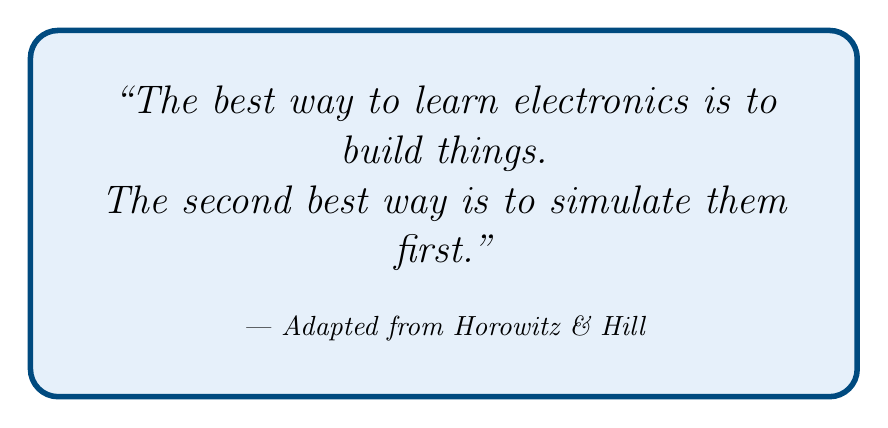
\begin{tikzpicture}
    \node[draw=primaryblue, line width=2pt, rounded corners=10pt, 
          inner sep=20pt, fill=lightblue] {
        \begin{minipage}{0.75\textwidth}
            \centering
            \Large\itshape
            ``The best way to learn electronics is to build things.\\
            The second best way is to simulate them first.''\\[1em]
            \normalsize
            --- Adapted from Horowitz \& Hill
        \end{minipage}
    };
\end{tikzpicture}
\end{center}

\vspace{2cm}

\begin{center}
    \textbf{\Large Document Summary}\\[0.5cm]
    \begin{tabular}{rl}
        \textbf{Total Circuits:} & 150+ \\
        \textbf{Development Phases:} & 6 \\
        \textbf{Estimated Timeline:} & 18--24 months \\
        \textbf{Primary Sources:} & AoE 3rd Edition, X Chapters \\
    \end{tabular}
\end{center}

\vspace*{\fill}

\end{document}
